\section{Introduction}

Machine learning techniques as a data analysis tool has been proving its efficiency in numerous research areas during the last decade.
The reason for such popularity is the core idea behind all of the employed methods -- inherent data pattern recognition.
Quantum physics seems a promising field for such tools since the size of data required to fully describe a system scales exponentially.

Active research is going in dense representation of states of quantum many-body systems, analysis of experimental data, state tomography and quantum chaos revealing.
Promising results was obtained in phase transition detection and several unique methods proposed.

In this paper, we generalize original learning by confusion algorithm to the case of 2 parameters for the GdFeCo system, get 3D accuracy surface as an analogue of $W$-shape and determine a bifurcation point.
Subsequent comparison with numerical results of classical approach allow to benchmark proposed approach.
Finally, we discuss further applications to the problem of amorphous ferrimagnets.

\section{Problem setting}

We are given \textcolor{red}{(how? Elaboration is required from Sergey)} the hamiltonian:

\begin{multline}
    H =
    -x\bm{M}_f\bm{H}_{eff}
    -(1-x)\bm{M}_d\bm{H}\\
    - xK_f\left(\frac{\bm{M}_f}{M_f}\bm{Z}\right)^2
    -(1-x)K_d\cos^2\theta_d\left(\frac{\bm{M}_d}{M_d}\bm{Z}\right)^2,
\end{multline}

where:
$\bm{H}$ -- external field,
$\bm{M}_{f,d}$ -- magnetization,
$\bm{H}_{eff} = \bm{H} - \lambda\bm{M}_d$,
$\bm{Z}$ -- anisotropy vector.

Let's introduce $\theta_d$ as an angle between $\bm{M}_d$ and $Z$.
In zero approximation $\bm{Z} || \bm{H}$ so we obtain:
\begin{multline}
    H =
    -xM_f H_{eff}-(1-x)M_d H\cos\theta_d\\
    - xK_f\left(\frac{\bm{M}_f}{M_f}\bm{Z}\right)^2
    -(1-x)K_d\cos^2\theta_d
\end{multline}

From physical observation we know that $\bm{M}_f = \chi_f \bm{H}_{eff}$, so:
\begin{equation}
    \frac{\bm{M}_f}{M_f}\bm{Z} =
    \frac{\bm{H}_{eff}}{H_{eff}}\bm{Z} =
    \frac{\bm{H} - \lambda\bm{M}_d}{H_{eff}}\bm{Z}=
    \frac{H - \lambda M_d \cos\theta_d}{H_{eff}}
\end{equation}
Defining the last expression as $\cos\theta_f$ we get:

\begin{multline}
    H = -xM_fH_{eff} -
    (1-x)M_dH\cos\theta_d -\\
    xK_f\cos^2\theta_f -
    (1-x)K_d\cos^2\theta_d
\end{multline}
With constants for the further computations set to:
    $\mu_{B} = 9.27\cdot10^{-21} \mathrm{erg}\cdot \mathrm{G}^{-1}$,
    $M_{f}=10 \mu_{B}$,
    $M_{d}=5 \mu_{B}$,
    $K_{d,f} = 2.55 \cdot 10^{-16}$,
    $\lambda = 10^5 \cdot \mu_{B}^{-1}$.



\section{Learning by confusion}
For phase transition identifying we use the method called "learning by confusion" originally proposed in \cite{VanNieuwenburg2017}.
It uses the data set that depends on some parameter $c$ that lies in the range $[c_0, c_1]$ and depict system properties.
Assuming that information about the current phase is encoded in this data we can teach the algorithm to categorise vectors into 2 groups.
These two groups would correspond to the system's phases.

However, it is unclear how to train the algorithm since we have no prior information about the proper phase attribution.
That is where learning by confusion enters to the scene.
We choose a parameter $c'\in[c_0, c_1]$, and set label $0$ to all the data with parameter value less then $c'$ and label $1$ to the rest.
By doing so we guess a critical parameter $c'$ and train the algorithm to learn hidden patterns in the data.
If our guess is correct, the algorithm would learn the hidden properties and predict phase attribution with high accuracy.
Otherwise, algorithm would be confused, would not learn any patterns and fail during the prediction phase.
Applying this procedure on the grid of $c'\in[c_0, c_1]$ we would observe the $W$-shape where central peak would depict the critical point.\footnote{If system has several phase transition points, number of peaks increase respectively}

In the case of GdFeCo, we have the data that depends on 2 parameters: $H$ and $x$.
For each set of parameters there is an angle $\theta_d$ at which energy minimum is reached.
This angle experiences a leap that indicates a phase transition to identify.
Thus we have 2 problems: 1) learning by confusion is originally designed only for 1 parameter;1) there is no information about the $\theta_d$ that provides the minimum;

The former problem is easily solved by the following approach.
We fix one parameter, say $H$, run the algorithm and get the corresponding $W$-shape.
Then we perform this step for the whole grid of $H$ and get a 2D surface where ridges show the phase transition lines.

Monte-Carlo inspired approach was applied to tackle the latter problem.
We sample $n_{\theta_d}$ angles $\theta_d \sim \mathcal{U}(0, \pi)$ for each set of parameters ($H$, $x$).
Then calculate hamiltonian values in each dot and find the angle $\hat{\theta_d}$ when energy is the smallest.
This estimation is our input vector for the following algorithm operations.

A few comments should be outlined considering the described approach.
The number $n_{\theta_d}$ should be tuned accurately because it has a significant effect on the algorithm precision.
During the experiments it was found that \textit{small} values of $n_{\theta_d}$ provides better results.
This is not obvious since the number of points at Monte-Carlo approaches is proportional to algorithms accuracy.

Moreover, the described data set building technique is not the only possible and was chosen to tackle the given problem.
For example, we tried to use the whole vector of energies for sampled $\theta_d$, but algorithm detected extreme number of phase transitions and an accuracy surface was almost a plane.
Finally, considering more complicated setting, one must look at PCA or any other dimensionality reduction solutions to handle the curse of dimensionality that naturally arises at such problems.


For model learning an \texttt{XGBoost} algorithm from \texttt{sklearn} library was used.
It is a powerful realisation of decision trees building algorithm.
Labeled data was split into 2 parts: \texttt{train} and \texttt{test}.
The first was used for model training while the second remained for accuracy computation and $W$-shape building.

For noise elimination, models (and corresponding $W$-shapes) was launched $n_{samples}$ times and then accuracy values were averaged.


\section{Theoretical predictions}\label{sec:theory}
\textcolor{red}{Sergey part?}

\section{Results}\label{sec:results}

\begin{figure*}[h]
    \centering
    \begin{minipage}{0.45\textwidth}
        \centering
        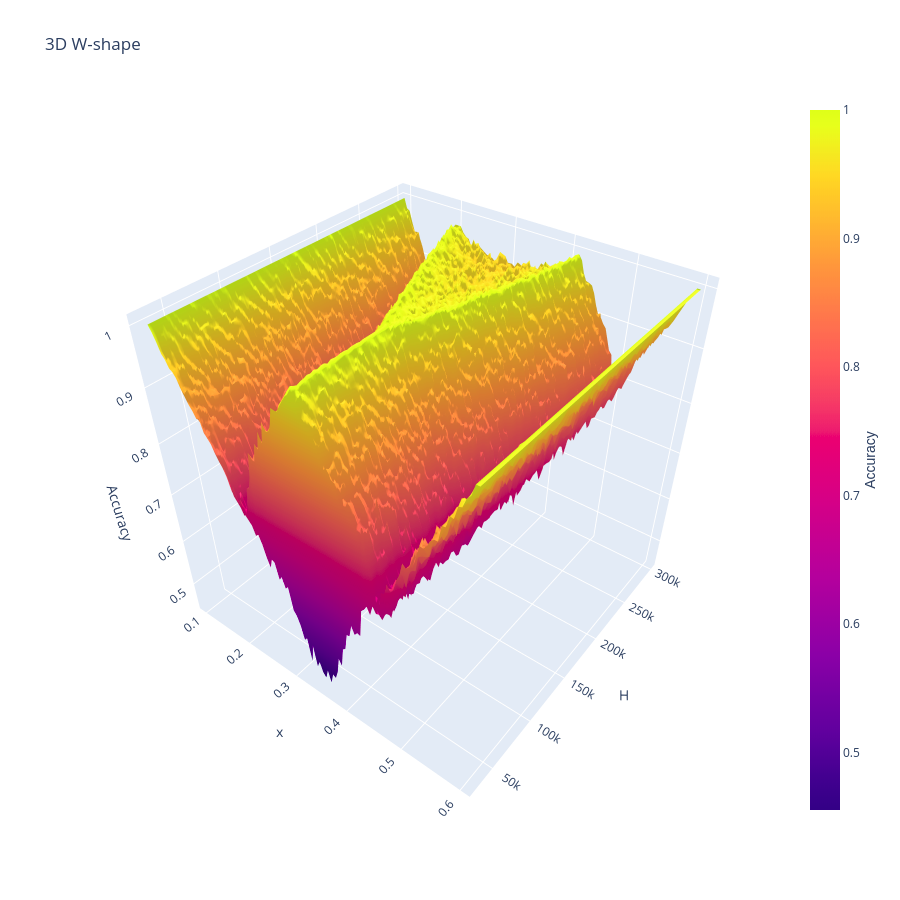
\includegraphics[width=0.9\textwidth]{../fig/wide_3D.png} % first figure itself
        \caption*{\textbf{a}}
        \label{fig:wide_3D}
    \end{minipage}\hfill
    \begin{minipage}{0.45\textwidth}
        \centering
        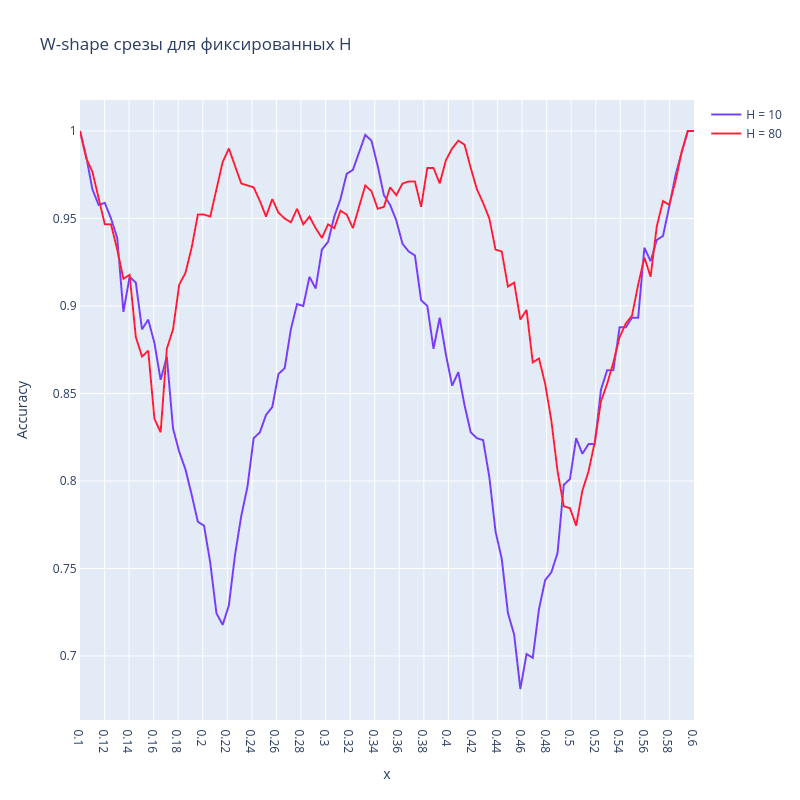
\includegraphics[width=0.9\textwidth]{../fig/wide_slices.png} % second figure itself
        \caption*{\textbf{b}}
        \label{fig:wide_slices}
    \end{minipage}
    \caption{Results of learning by confusion algorithm for $x \in \{0.1, 0.6\}$ and $H \in \{0, 3 \cdot 10^5\}$. \textbf{a.} 3D view of a W-shape structure. Lines of phase transition are clearly observed as a ridge on the accuracy surface. \textbf{b.} 2 slices that represent w-shape for particular fixed points of $H$. Despite the fluctuations, peaks with high accuracy values are easily distinguished.}
    \label{fig:wide}
\end{figure*}

Applying the described approach to the wide range of parameters we observed the general view of phase transition lines.
For $ \in \{0.1, 0.6\}$ and $H \in \{0, 3 \cdot 10^5\}$ we got the results shown in Fig \ref{fig:wide}.
Fig \ref{fig:wide_3D} depicts a bird view on the accuracy surface.
Bifurcating phase transition line was clearly found by the algorithm.
The novelty of this result comparing to the existing works consists of the discovery of generalized $W$-shape either in terms of multiple parameters, or in terms of nontrivial peaks topology.\textcolor{red}{['topology'?? Should be rewritten]}.
Several fixed points of $H$ was chosen to demonstrate original $W$-shape on the Fig. \ref{fig:wide_slices}.
One can see that despite the fluctuations, points with highest accuracies stands out rather sharp.
That allows to determine phase transition with high precision.

\begin{figure*}
    \centering
    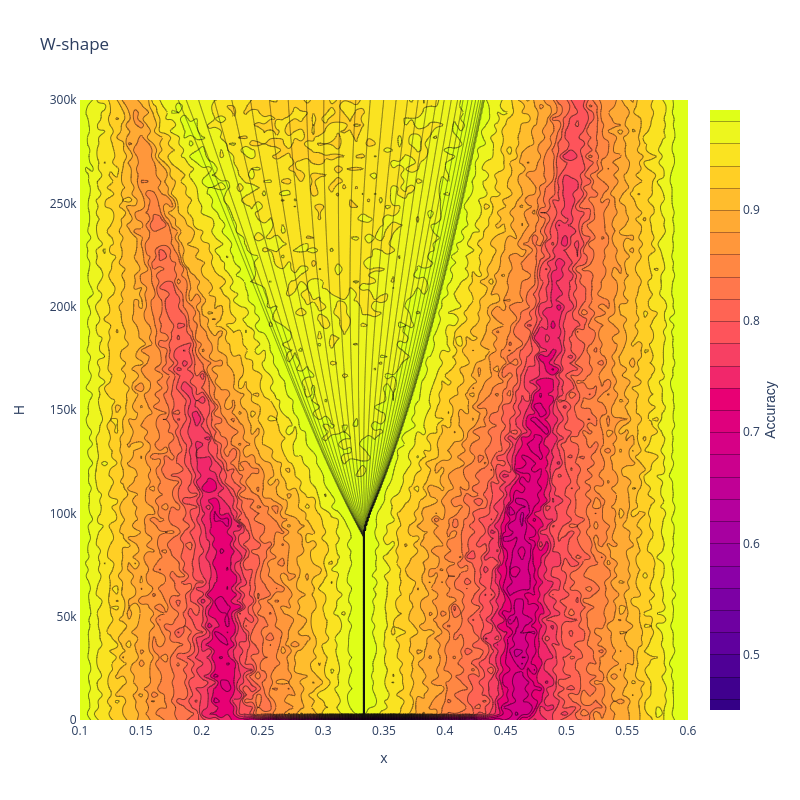
\includegraphics[width=0.5\textwidth]{../fig/wide_2D.png}
    \caption{Heatmap of the learning by confusion algorithm results (colored) and numerical calculations of phase transition lines (black).}
    \label{fig:wide_2D}
\end{figure*}

Classical numerical approach was used to calculate regions of phase transition.
Comparison it with the results of the proposed algorithm shows the exact match(Fig \ref{fig:wide_2D})
It can be viewed as a good indicator of the method quality.

We also considered a narrowed intervals of parameters to better observe bifurcation point.
The results are shown in Fig. \ref{fig:bifurcation}

\begin{figure*}[h]
    \centering
    \begin{minipage}{0.45\textwidth}
        \centering
        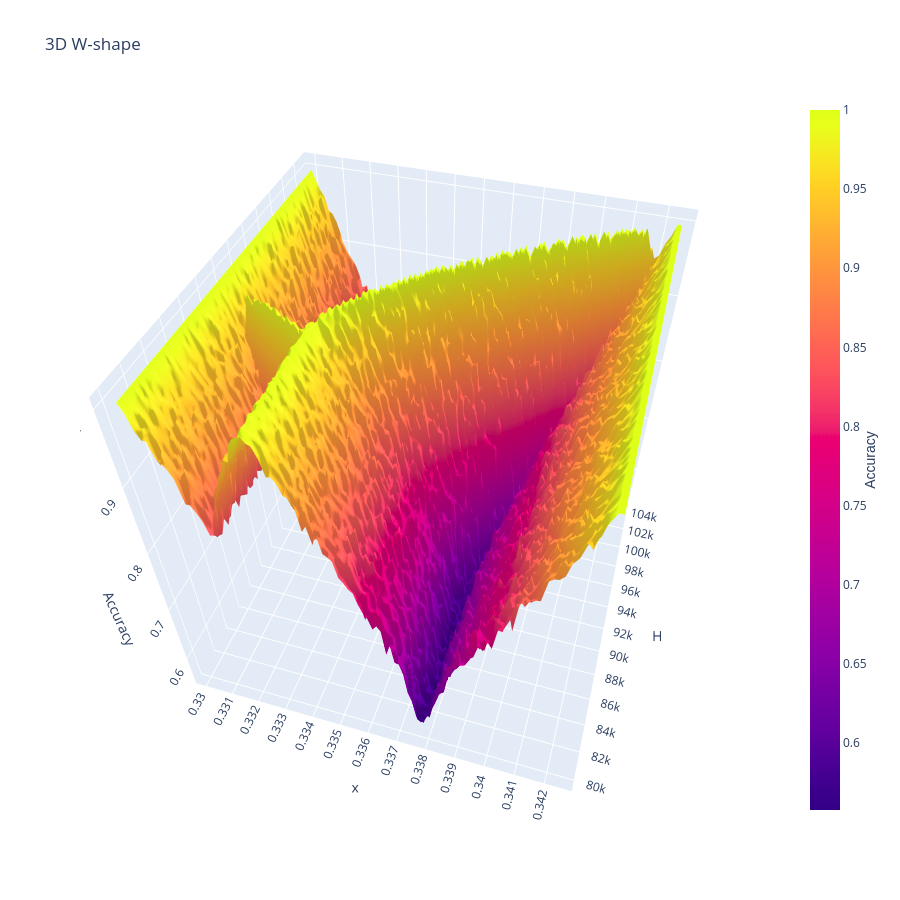
\includegraphics[width=0.9\textwidth]{../fig/bifurcation_3D.png} % first figure itself
        \caption*{\textbf{a}}
        \label{fig:narrow_3D}
    \end{minipage}\hfill
    \begin{minipage}{0.45\textwidth}
        \centering
        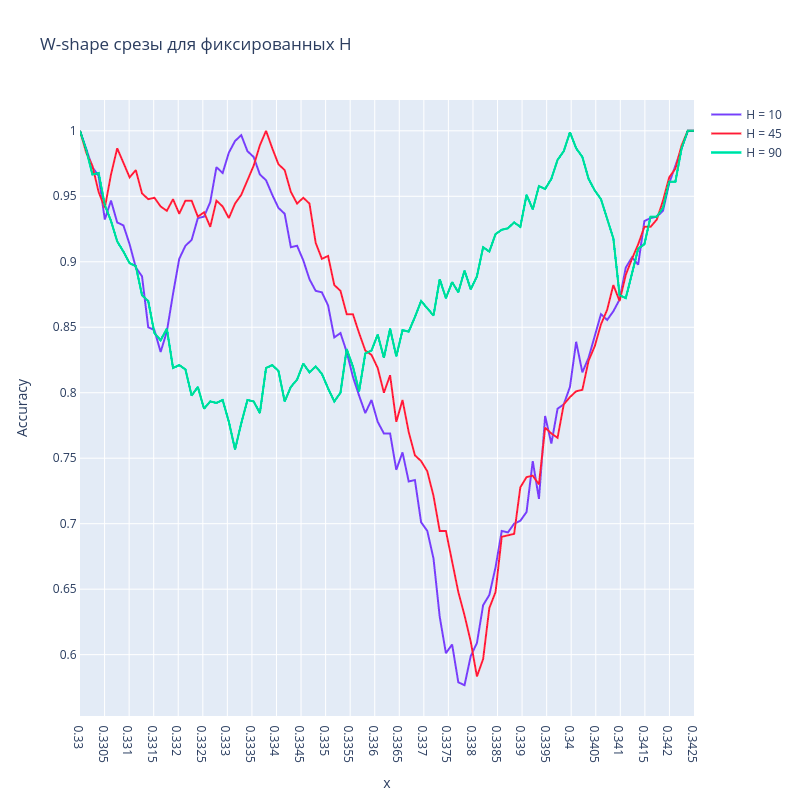
\includegraphics[width=0.9\textwidth]{../fig/bifurcation_slices.png} % second figure itself
        \caption*{\textbf{b}}
        \label{fig:narrow_slices}
    \end{minipage}
    \caption{Results of learning by confusion algorithm for $x \in \{0.33, 0.3425\}$ and $H \in \{0.8 \cdot 10^5, 1.05 \cdot 10^5\}$. \textbf{a.} 3D view of a W-shape structure. Lines of phase transition are clearly observed as a ridge on the accuracy surface. \textbf{b.} 2 slices that represent w-shape for particular fixed points of $H$. Despite the fluctuations, peaks with high accuracy values are easily distinguished.}
    \label{fig:bifurcation}
\end{figure*}

\section{Discussions}\label{Discussions}
We proposed an adaptation of the learning by confusion method for the problem of phase transition detection in the weak ferromagnetic GdFeCo.
It generalizes the original algorithm to the case of 2 parameter dependence.
Moreover, since several phase areas are present, $W$-shape transforms to the more complicated figure.

The results of the described approach shows a good correspondence with transition lines obtained from classical numerical algorithms.
Thus this method can be used for amorphous ferrimagnets, where anisotropy vector varies from site to site.\textcolor{red}{[hope I understand it correctly]}.
For this purpose novel approaches to dataset generation should be considered.
